\documentclass[12pt]{article}
\usepackage[margin=1in]{geometry}
\usepackage{amsmath,amssymb,booktabs,tabularx,graphicx,setspace,longtable}
\usepackage{xurl}
\usepackage[colorlinks=true,citecolor=blue,linkcolor=blue,urlcolor=black]{hyperref}
\singlespacing
\setlength{\emergencystretch}{2em}
\graphicspath{{figures/}}
\begin{document}
\begin{center}
{\Large \textbf{Supporting Information}}\\[0.5em]
{\large Forecast Evaluation with Constructed High-Frequency Targets: Information-Set Leakage and an African Gross Domestic Product Application}
\end{center}

\section{News-source registry and web collection}
The source registry contains 851 distinct newspaper and digital-news outlets covering all 54 African economies. Each registry record contains an outlet name, country, language label, and website. The median country has 13 registered sources, with a range from 2 to 66. The source universe is multilingual: English and French are the largest groups, with dedicated Arabic- and Portuguese-language outlets and additional national, regional, and multilingual sources. Registered sources need not be available in every month, so source counts are treated as an upper-level coverage frame rather than a balanced monthly panel.

Collection is implemented as a recurring country--newspaper--month web-scraping process. Raw article files contain titles and article text. Retrieval is monitored at the source-month level. A source returning at least 20 percent fewer articles than in the preceding month enters scheduled retry passes. Only the strongest successful scrape for a newspaper-month is retained; multiple attempts are never concatenated. Cross-source duplicate screening is applied during collection, and completed monthly data are promoted to the historical archive only after the collection and processing stages complete successfully. These rules are designed to separate genuine changes in news volume from temporary website failures, incomplete retrieval, and repeated requests.

The frozen analytical archive contains 21,303,573 retained article records from January 2015 through December 2025. A total of 5,896,776 records satisfy the economic-relevance rule. The archive contains 7,127 country-month observations; 6,488 have at least 100 retained articles and the median country-month contains 1,039 records. Missing or unreadable source-months remain distinguishable from observed months with no qualifying risk content.

The unit of measurement is an article record, not an inferred independent news event. Cross-source screening cannot eliminate every syndicated, translated, or edited copy. A reconstructed exact-text audit removes 497,091 repeated records (2.33 percent), including 186,379 exact copies appearing across outlets. The forecast signal uses the frozen production vintage; the duplicate audit is reported as a corpus-quality diagnostic rather than substituted ex post for the measured signal.

\begin{table}[htbp]
\centering
\caption{News-source registry summary}
\begin{tabular}{lr}
\toprule
Registered newspaper and digital-news sources & 851\\
African economies covered & 54\\
Median registered sources per country & 13\\
Minimum registered sources in a country & 2\\
Maximum registered sources in a country & 66\\
Retained article records, 2015--2025 & 21,303,573\\
Economically relevant records & 5,896,776\\
Country-month observations & 7,127\\
Country-months with at least 100 articles & 6,488\\
\bottomrule
\end{tabular}
\end{table}

Figure~\ref{fig:coverage} reports the number of countries with at least 100 retained articles by month.
\begin{figure}[htbp]
\centering
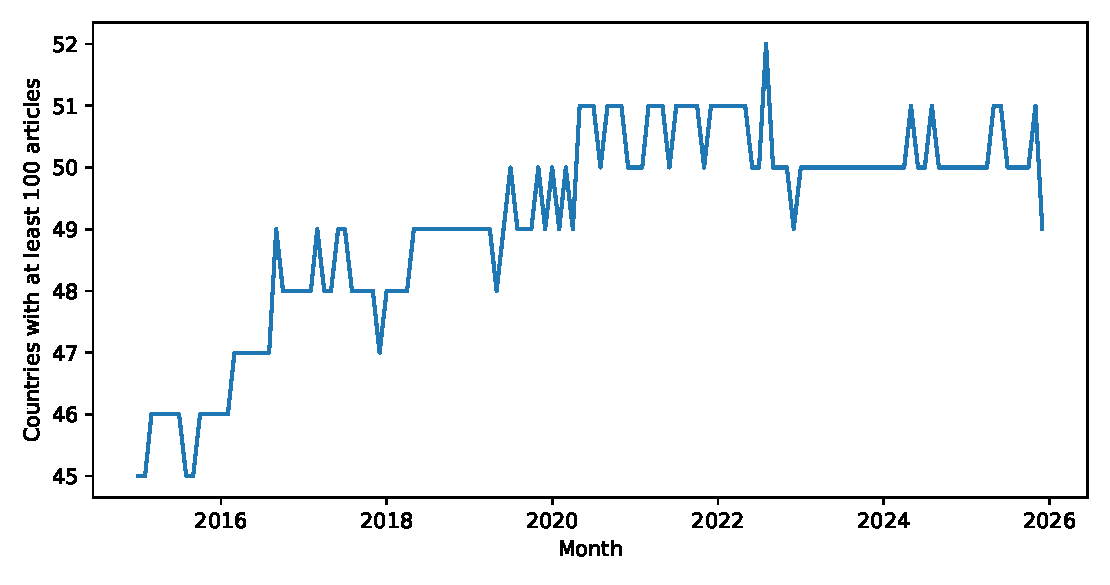
\includegraphics[width=0.82\textwidth]{Supplement_Figure_Coverage.pdf}
\caption{Monthly news-coverage diagnostic.}
\label{fig:coverage}
\end{figure}

A GRE archive-depth regression over the 6,488 country-months satisfying the 100-article criterion gives a log-article-volume coefficient of 0.103 with country fixed effects ($p=0.656$), and 0.100 with both country and month fixed effects ($p=0.713$). These diagnostics do not establish source representativeness but provide little evidence of a mechanical within-country relation between GRE and archive size.



\section{Growth/Real Economy signal construction}
The main paper keeps the news variable brief because the forecast-design issue does not depend on the details of the text score. This section records the construction used in the African application.

For article $i$, let $x_i$ denote normalized headline and body text. Economic relevance is
\begin{equation}
R_i=\mathbf{1}\{x_i \text{ matches the economic-relevance dictionary}\}.
\end{equation}
Articles that do not pass this screen receive zero score but remain in the country-month denominator. The Growth/Real Economy activation indicator is
\begin{equation}
G_i=\mathbf{1}\{x_i \text{ activates the Growth/Real Economy dictionary}\}.
\end{equation}
The production vocabulary includes recession, slowdown, contraction, unemployment, layoffs, and corresponding French and Portuguese terms. Broader words such as GDP and growth belong to the economic-relevance screen rather than the target-specific activation rule.

Relevant articles receive an ordinal severity score,
\begin{equation}
S_i=\begin{cases}
0,&R_i=0,\\
\max(\{1\}\cup\mathcal K_i),&R_i=1,
\end{cases}
\end{equation}
where $\mathcal K_i\subseteq\{1,2,3,4\}$ contains the matched severity tiers. Tier 1 records mild or background pressure, tier 2 material deterioration, tier 3 severe disruption, and tier 4 extreme or systemic stress.

Textual emphasis uses a headline cue $T_i$, a body-length indicator $L_i$ for at least 1,200 normalized characters, and $M_i$ for articles activating at least two economic domains:
\begin{equation}
W_i=\operatorname{clip}(1+0.5T_i+0.2L_i+0.3M_i,1,2).
\end{equation}
These coefficients are fixed and are not estimated from GDP. The article contribution is
\begin{equation}
Q_i=R_iG_iS_iW_i.
\end{equation}
For country $c$ and month $t$, with retained article set $\mathcal A_{ct}$ and $N_{ct}=|\mathcal A_{ct}|$,
\begin{equation}
GRE_{ct}=\frac{100}{N_{ct}}\sum_{i\in\mathcal A_{ct}}R_iG_iS_iW_i.
\end{equation}
Keeping all retained articles in the denominator means GRE rises when real-economy risk coverage becomes more common, more severe, or more prominent in the observed news flow. The scoring rule is fixed before forecast evaluation and is not tuned by searching for low GDP forecast loss.

\begin{table}[htbp]
\centering\small
\caption{Construction of the Growth/Real Economy news signal}
\label{tab:construction}
\begin{tabularx}{\textwidth}{p{0.19\textwidth}X}
\toprule
Stage & Definition and interpretation \\
\midrule
Economic relevance $R_i$ & Indicator that normalized article text contains economically relevant content. Articles failing this screen contribute zero to the signal but remain in the country-month denominator. \\
Real-economy activation $G_i$ & Indicator that the article activates the frozen Growth/Real Economy dictionary: recession, slowdown, contraction, unemployment, layoffs, and the corresponding French and Portuguese activation terms. Broader GDP/growth vocabulary belongs to the economic-relevance screen rather than this target-specific activation rule. \\
Severity $S_i$ & Ordinal score for relevant articles: 1 = background or mild pressure; 2 = material deterioration; 3 = severe disruption; 4 = extreme or systemic real-economy stress. The highest matched tier applies. \\
Textual emphasis $W_i$ & $\operatorname{clip}(1+0.5T_i+0.2L_i+0.3M_i,1,2)$, where $T_i$ marks headline emphasis, $L_i$ marks at least 1,200 normalized characters, and $M_i$ marks economically dense multi-domain content. \\
Article contribution $Q_i$ & $Q_i=R_iG_iS_iW_i$. Only economically relevant articles that activate the real-economy domain contribute positive weight. \\
Country-month signal $GRE_{ct}$ & $100N_{ct}^{-1}\sum_{i\in\mathcal A_{ct}}Q_i$, where $N_{ct}$ is the total number of retained articles. The signal therefore reflects both the prevalence and the intensity of real-economy risk reporting. \\
\bottomrule
\end{tabularx}
\end{table}

\begin{table}[htbp]
\centering\scriptsize
\caption{Illustrative article-level mapping into the Growth/Real Economy signal}
\label{tab:worked_example}
\begin{tabularx}{\textwidth}{p{0.32\textwidth}cccccX}
\toprule
Stylized article content & $R_i$ & $G_i$ & $S_i$ & $W_i$ & $Q_i$ & Interpretation \\
\midrule
``Manufacturing output contracts sharply; factories announce layoffs and demand weakens'' & 1 & 1 & 3 & 2.0 & 6.0 & Economically relevant, activates the real-economy domain, severe language, and high textual emphasis. \\
``Foreign-exchange reserves decline while the currency comes under pressure'' & 1 & 0 & -- & -- & 0 & Economically relevant but does not activate the Growth/Real Economy domain, so it does not enter this signal. \\
Sports or entertainment article with no economic content & 0 & 0 & 0 & -- & 0 & Retained in the monthly article denominator but contributes zero to the numerator. \\
\bottomrule
\end{tabularx}
\vspace{0.3em}
\begin{minipage}{0.96\textwidth}\footnotesize\textit{Notes:} Examples are stylized illustrations, not quotations from the archive. For the first row, $W_i$ reaches its upper bound when all three emphasis indicators are active.\end{minipage}
\end{table}


Figure~\ref{fig:gre_descriptive_supp} plots the monthly cross-country median and interquartile range. Coverage varies over time, so the forecast analysis uses separate minimum-article and exact-text checks rather than assuming a balanced media panel.
\begin{figure}[htbp]
\centering
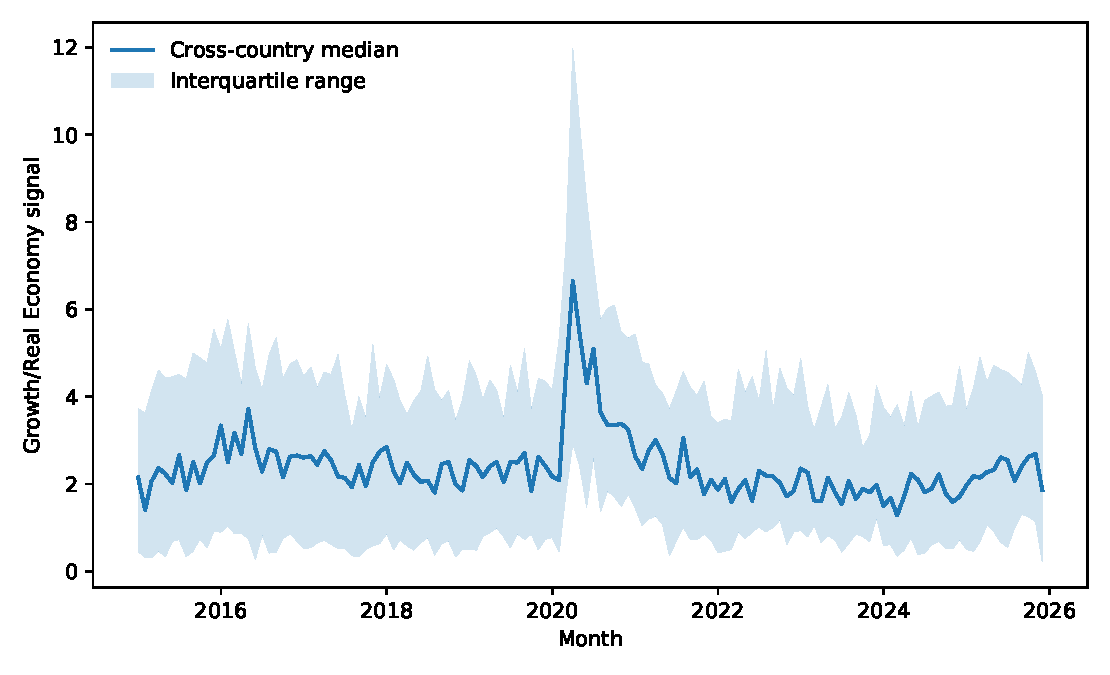
\includegraphics[width=0.82\textwidth]{Figure_0_GRE_Descriptive.pdf}
\caption{Cross-country distribution of the Growth/Real Economy news signal, 2015--2025.}
\label{fig:gre_descriptive_supp}
\end{figure}

The closest construction-based comparator is broad AERI, which uses the same relevance, severity, and emphasis rules but does not require the real-economy domain indicator. Inflation Risk and FX/External Risk are used as additional falsification comparators in the forecast exercise. None of these alternatives is used to select or tune GRE.

\section{GDP-PPP data provenance and target-information audit}
The annual activity input is the exact series labeled ``GDP (PPP)-WEO'' in the author-supplied workbook \nolinkurl{GDP_Data_African_countries_AUTHOR_SUPPLIED_2026-09-13.xlsx}. The replication package freezes that workbook as supplied on 13 September 2026 and provides the cleaned country-year extract \nolinkurl{annual_gdp_ppp_weo_labeled_final_vintage_2015_2025.csv}. The workbook does not contain an IMF WEO publication-release identifier. We treat the observations as final-vintage WEO-labeled data and do not claim that they reproduce the historical values available to forecasters at each origin.

The final-vintage monthly evaluation target is constructed by additive first-difference Denton. If $Y_c$ stacks annual benchmarks, $G_c^F$ stacks monthly values, $D$ is the first-difference operator, and $A$ maps months into annual sums, then
\[
\min_{G_c^F}(DG_c^F)'(DG_c^F)\quad\text{subject to}\quad AG_c^F=Y_c.
\]
The monthly values reaggregate exactly to the annual benchmarks. The realized target is $100[\log G^F_{ct}-\log G^F_{c,t-12}]$.

The critical information-timing distinction is that $G_c^F$ is \emph{not} supplied to the forecasting model as if it had been observed historically. For every forecast origin the script reconstructs a separate GDP history from annual benchmark years allowed by the release convention. Under the baseline May rule, annual year $y$ is not available until May of $y+1$. Denton is applied only through the most recent permitted annual year; months after that year and through the forecast origin are extrapolated at the log-monthly rate implied by the two most recent permitted annual totals. A target dated in year $y$ cannot enter the recursive training sample before May of $y+1$.

For example, at a January 2020 forecast origin the May rule permits annual benchmarks only through 2018, whereas a June 2020 origin permits 2019. The November sensitivity rule is more conservative: annual 2019 does not enter until November 2020. These rules prevent the 2020--2025 annual totals from mechanically shaping GDP lags before their assumed release dates.

The procedure still uses final-vintage values for annual years deemed released. It does not remove revisions to previously released years. A genuine historical-vintage experiment would require archived country-level annual GDP vintages and release calendars for every economy. The revised manuscript states this limitation explicitly and uses the term ``publication-lagged final-vintage'' rather than ``real time'' or ``leakage-free.''


\section{Closed-form Denton weight characterization}
This section supplies the algebra behind Proposition 1 in the main paper. The result concerns the interior behavior of additive first-difference Denton with twelve months per annual block. It is a characterization of the linear disaggregation operator, not an additional empirical assumption.

Fix one year and write $p=e_{y-1}$ and $q=e_y$ for the monthly levels at the preceding and current year-end. Let $d_1,\ldots,d_{12}$ be the monthly first differences and $x_i=p+\sum_{j\leq i}d_j$ the within-year monthly levels. The two constraints are
\[
\sum_{i=1}^{12}d_i=q-p,
\qquad
12p+\sum_{i=1}^{12}(13-i)d_i=Y_y.
\]
With
\[
C=\begin{pmatrix}
1&\cdots&1\\
12&11&\cdots&1
\end{pmatrix},
\qquad
b=\begin{pmatrix}q-p\\Y_y-12p\end{pmatrix},
\]
the minimum-norm solution is $d=C'(CC')^{-1}b$. Here
\[
CC'=\begin{pmatrix}12&78\\78&650\end{pmatrix},
\qquad
(CC')^{-1}=\begin{pmatrix}25/66&-1/22\\-1/22&1/143\end{pmatrix}.
\]
The minimized within-year roughness is therefore
\begin{equation}
R(p,q,Y)
=\frac{Y^2}{143}-\frac{Yp}{13}-\frac{Yq}{11}
 +\frac{23p^2}{78}+\frac{pq}{3}+\frac{25q^2}{66}.
\label{eq:s_R}
\end{equation}

The full Denton problem reduces to minimizing $\sum_y R(e_{y-1},e_y,Y_y)$ over the year-end sequence. Differentiating the two adjacent block contributions with respect to an interior $e_y$ gives
\begin{equation}
\frac{1}{3}e_{y-1}+\frac{578}{429}e_y+\frac{1}{3}e_{y+1}
=\frac{Y_y}{11}+\frac{Y_{y+1}}{13}.
\label{eq:s_boundary_recursion}
\end{equation}
The associated homogeneous characteristic equation is
\[
\frac{1}{3}+\frac{578}{429}z+\frac{1}{3}z^2=0,
\]
with roots
\[
\mu=\frac{12\sqrt{438}-289}{143}\approx-0.2647454934,
\qquad
\mu^{-1}\approx-3.7772125485.
\]
Because the two off-diagonal coefficients in equation~\eqref{eq:s_boundary_recursion} are equal, the roots are reciprocal. The bounded doubly-infinite solution retains only $\mu$ in the tail. A benchmark $Y_s$ enters the right-hand side of equation~\eqref{eq:s_boundary_recursion} only at two adjacent annual boundary equations, so outside those directly forced blocks its effect on $e_y$ is proportional to $\mu^{|y-s|}$.

Back-substitution provides the exact within-year interpolation formula. For month $r\in\{1,\ldots,12\}$,
\begin{equation}
x_{y,r}
= a_r e_{y-1}+b_r e_y+c_rY_y,
\qquad
a_r=\frac{(r-12)(3r-13)}{156},\quad
b_r=\frac{r(3r-25)}{132},\quad
c_r=\frac{r(12-r)}{286}.
\label{eq:s_monthly_backsub}
\end{equation}
Hence the annual-benchmark weights inherited by any interior month also have geometric off-diagonal tails. In particular, for a month $t=(y_0,r)$ there are constants $C_r^+$ and $C_r^-$ such that
\[
H_{t,y_0+k}=C_r^+\mu^{k-1},\qquad
H_{t,y_0-k}=C_r^-\mu^{k-1},\qquad k\geq1.
\]
The constants differ by month because the first off-diagonal exposure is determined by equation~\eqref{eq:s_monthly_backsub}. This distinction matters: $|\mu|$ is the exact ratio between successive tail coefficients, not a universal ratio of the first future-year coefficient to the own-year coefficient.

\begin{table}[htbp]
\centering\scriptsize
\caption{Interior within-year Denton benchmark-weight profile}
\label{tab:s_denton_profile}
\begin{tabular}{rrrrr}
\toprule
Month $r$ & Own-year $H_{t,y_0}$ & Next-year $H_{t,y_0+1}$ & $|H_{t,y_0+1}/H_{t,y_0}|$ & $H_{t,y_0+2}/H_{t,y_0+1}$ \\
\midrule
1  & 0.06025 & -0.01595 & 0.26475 & -0.26475 \\
2  & 0.07284 & -0.01836 & 0.25204 & -0.26475 \\
3  & 0.08291 & -0.01917 & 0.23125 & -0.26475 \\
4  & 0.09047 & -0.01840 & 0.20335 & -0.26475 \\
5  & 0.09550 & -0.01603 & 0.16782 & -0.26475 \\
6  & 0.09802 & -0.01207 & 0.12309 & -0.26475 \\
7  & 0.09802 & -0.00651 & 0.06643 & -0.26475 \\
8  & 0.09550 &  0.00063 & 0.00665 & -0.26475 \\
9  & 0.09047 &  0.00937 & 0.10361 & -0.26475 \\
10 & 0.08291 &  0.01970 & 0.23765 & -0.26475 \\
11 & 0.07284 &  0.03163 & 0.43420 & -0.26475 \\
12 & 0.06025 &  0.04514 & 0.74925 & -0.26475 \\
\bottomrule
\end{tabular}
\begin{singlespace}\footnotesize\textit{Notes:} Interior, doubly-infinite characterization for additive first-difference Denton with 12 months per annual block. The own-year and next-year columns are weights on annual totals in a monthly value, with each row satisfying $\sum_y H_{t,y}=1/12$ after all annual blocks are included. The first unavailable-year exposure is month-specific; the exact constant decay rate applies to successive off-diagonal tail coefficients.\end{singlespace}
\end{table}


The table shows that first-future-year exposure can be small or substantial depending on the month and can change sign within the year. Once that first off-diagonal term is fixed, however, the next annual coefficient is always $\mu$ times the preceding one in the interior solution. The negative root therefore generates alternating signs, while $|\mu|<1$ produces rapid attenuation.

As a finite-sample check, the replication package reconstructs the exact 132-month Denton map for the 2015--2025 sample and compares successive off-diagonal ratios with the interior root. For a central 2018 annual block, the first and second future-tail ratios differ from $\mu$ by approximately $1.1\times10^{-7}$ and $1.6\times10^{-6}$, respectively; deviations grow as the opposite sample boundary is approached. The files \nolinkurl{GDP_Construction/denton_weight_characterization/denton_interior_month_profile.csv}, \nolinkurl{denton_geometric_decay.csv}, and \nolinkurl{denton_finite_sample_crosscheck.csv}, together with \nolinkurl{verify_denton_weight_decay.py}, reproduce the calculations.

\section{Monte Carlo design and full simulation results}
The Monte Carlo exercise isolates target-information treatment from the institutional details of the African application. Each replication contains 54 economies from 2015 through 2025, annual GDP is temporally disaggregated with the same first-difference Denton operator used in the paper, and the benchmark conditions on three lags of twelve-month growth and country fixed effects. The retrospective design supplies the complete final-vintage Denton history; the publication-lagged design admits annual year $y$ only from May of $y+1$.

Three DGPs are reported. The \emph{current-state signal} is intentionally modest: the alternative variable measures the contemporaneous annual activity innovation with noise and contains no next-year innovation. It is calibrated to produce a small feasible short-horizon gain. The \emph{pure-noise placebo} replaces the signal with independent noise. The \emph{persistent-state stress} DGP raises annual persistence from 0.25 to 0.95 and increases the signal-to-noise ratio. It is chosen only to establish an existence result in which the retrospective design generates the same direction of 12-month reversal observed in the African data. It is not intended to match the full empirical horizon profile or identify the mechanism generating the empirical reversal.

\begin{table}[htbp]
\centering\scriptsize
\caption{Full Monte Carlo results across three DGPs}
\begin{tabular}{llrrr}
\toprule
DGP & Design & $h$ & Mean rel. RMSFE & Share $<1$\\
\midrule
Current-state & Retrospective & 1 & 1.0002 & 39.0\%\\
Current-state & Publication-lagged & 1 & 0.9969 & 97.7\%\\
Current-state & Retrospective & 3 & 1.0002 & 36.6\%\\
Current-state & Publication-lagged & 3 & 0.9973 & 96.5\%\\
Current-state & Retrospective & 6 & 1.0002 & 39.2\%\\
Current-state & Publication-lagged & 6 & 0.9987 & 84.6\%\\
Current-state & Retrospective & 12 & 1.0001 & 47.5\%\\
Current-state & Publication-lagged & 12 & 1.0025 & 47.6\%\\
\midrule
Persistent-state stress & Retrospective & 1 & 1.0042 & 12.3\%\\
Persistent-state stress & Publication-lagged & 1 & 0.8715 & 100.0\%\\
Persistent-state stress & Retrospective & 3 & 1.0024 & 10.1\%\\
Persistent-state stress & Publication-lagged & 3 & 0.8793 & 100.0\%\\
Persistent-state stress & Retrospective & 6 & 0.9990 & 73.2\%\\
Persistent-state stress & Publication-lagged & 6 & 0.9149 & 100.0\%\\
Persistent-state stress & Retrospective & 12 & 0.9962 & 90.2\%\\
Persistent-state stress & Publication-lagged & 12 & 1.0122 & 35.1\%\\
\midrule
Pure-noise placebo & Retrospective & 1 & 1.0002 & 34.5\%\\
Pure-noise placebo & Publication-lagged & 1 & 1.0001 & 42.0\%\\
Pure-noise placebo & Retrospective & 12 & 1.0001 & 43.1\%\\
Pure-noise placebo & Publication-lagged & 12 & 1.0015 & 46.5\%\\
\bottomrule
\end{tabular}
\end{table}

The two signal DGPs deliberately demonstrate different distortions. In the modest current-state DGP, retrospective final-vintage history largely suppresses feasible short-horizon value and does not create a 12-month gain. In the persistent-state stress DGP, the 12-month retrospective ratio falls to 0.9962 while the publication-lagged ratio rises to 1.0122, reproducing the direction of the empirical reversal. The stress design's much larger short-horizon effects show why it should not be read as an empirical calibration. The pair of simulations supports the general admissibility result: the sign and horizon location of the distortion depend on persistence, signal strength, and how the constructed target enters the benchmark. The placebo shows that the procedure does not mechanically turn unrelated noise into a useful predictor.

\section{Publication-lagged horizon profile}
The baseline results use the May release convention, 2015--2018 frozen text scaling, and January 2020--December 2025 target dates.
\begin{table}[htbp]
\centering\scriptsize
\caption{Full horizon profile under the May release convention}
\begin{tabular}{rrrrrrrr}
\toprule
$h$ & Benchmark RMSFE & GRE RMSFE & Rel. RMSFE & Rel. MAE & HAC CW $p$ & Two-way $p$ & Target months\\
\midrule
1 & 8.375 & 8.344 & 0.9964 & 0.9897 & 0.0006 & 0.053 & 72\\
3 & 8.493 & 8.473 & 0.9977 & 0.9928 & 0.041 & 0.084 & 72\\
6 & 8.588 & 8.620 & 1.0037 & 1.0028 & 0.878 & 0.869 & 72\\
12 & 19.264 & 19.357 & 1.0048 & 1.0122 & 0.905 & 0.872 & 72\\
\bottomrule
\end{tabular}
\end{table}

Holm correction across the four target-month HAC values gives adjusted $p=0.0023$ at one month and 0.122 at three months. The corresponding two-way adjusted values are 0.211 and 0.253. The target-month aggregation gives the strongest result and directly preserves the contemporaneous country cross-section; the two-way calculation is a complementary, more conservative diagnostic in the baseline May specification.

\section{Release-month sensitivity}
\begin{table}[htbp]
\centering\scriptsize
\caption{One-month result under alternative annual-data release conventions}
\begin{tabular}{lrrrrrr}
\toprule
Release convention & Rel. RMSFE & Rel. MAE & HAC CW $p$ & Two-way $p$ & Bootstrap CW $p$ & Countries improved\\
\midrule
May of $y+1$ & 0.9964 & 0.9897 & 0.0006 & 0.053 & 0.037 & 33/54\\
July of $y+1$ & 0.9969 & 0.9894 & 0.0004 & 0.039 & 0.038 & 31/54\\
November of $y+1$ & 0.9973 & 0.9910 & 0.0001 & 0.030 & 0.019 & 32/54\\
\bottomrule
\end{tabular}
\end{table}

The direction of the one-month comparison survives progressively more conservative release rules. The raw point gain becomes smaller as annual information is withheld longer, but MAE remains approximately one percent below the benchmark and the dependence-aware test results remain favorable.

\section{Block-bootstrap uncertainty}
The moving-block bootstrap resamples 12-month target-date blocks and preserves the contemporaneous country cross-section. Under the May rule, the one-month raw RMSFE improvement is 0.362 percent. Across 5,000 replications, 82.6 percent of draws are positive, the 90 percent interval is approximately $[-0.34,1.31]$ percent, the 95 percent interval is $[-0.50,1.44]$ percent, and the one-sided bootstrap probability for a non-positive Clark--West mean is 0.037. Adjusted-loss inference is favorable, while the raw RMSFE improvement remains imprecisely estimated.

At 12 months, the corrected May-rule comparison is unfavorable: the actual RMSFE improvement is $-0.484$ percent and the bootstrap distribution is concentrated below zero. We make no long-horizon forecast-improvement claim.

\section{Domain-alignment comparison}
At one month, GRE is compared with broad AERI, Inflation Risk, and FX/External Risk under the identical publication-lagged benchmark.
\begin{table}[htbp]
\centering\scriptsize
\caption{Text comparators under the corrected one-month design}
\begin{tabular}{lrrrrr}
\toprule
Signal & Rel. RMSFE & Rel. MAE & HAC CW $p$ & Two-way $p$ & Raw-loss direction\\
\midrule
GRE & 0.9964 & 0.9897 & 0.0006 & 0.053 & Improves\\
Broad AERI & 1.0024 & 1.0020 & 0.0003 & 0.238 & Worsens\\
Inflation Risk & 1.0153 & 1.0225 & 1.000 & 0.992 & Worsens\\
FX/External Risk & 1.0003 & 0.9980 & $<0.001$ & 0.208 & Mixed / essentially neutral\\
\bottomrule
\end{tabular}
\end{table}

The Clark--West adjustment can be favorable even when unadjusted MSE is slightly higher, because it corrects the nested-model loss differential for the estimated augmentation. We do not treat a small Clark--West $p$-value as sufficient evidence of improvement when relative RMSFE exceeds one. GRE is the only signal in this restricted set that reduces both RMSFE and MAE.


\section{Information-staleness and revision diagnostics}
The short-horizon interpretation in the main paper motivates two direct diagnostics. First, each release convention is split into forecast origins before and after the assumed annual-data release month. The results are:
\begin{table}[htbp]
\centering\scriptsize
\caption{One-month GRE performance by annual-information state}
\begin{tabular}{llrrrr}
\toprule
Release rule & State & Target months & Rel. RMSFE & Rel. MAE & HAC CW $p$\\
\midrule
May & Stale pre-release & 24 & 0.9925 & 0.9804 & 0.0008\\
May & Refreshed post-release & 48 & 0.9985 & 0.9947 & 0.0286\\
July & Stale pre-release & 36 & 0.9937 & 0.9815 & 0.0001\\
July & Refreshed post-release & 36 & 1.0010 & 0.9984 & 0.1432\\
November & Stale pre-release & 60 & 0.9975 & 0.9907 & 0.0005\\
November & Refreshed post-release & 12 & 0.9961 & 0.9926 & 0.0574\\
\bottomrule
\end{tabular}
\end{table}
The May and July conventions display the pattern expected if news is more useful when the latest annual benchmark is stale. The November split does not preserve the same RMSFE ordering and contains only 12 post-release target months. The pattern is suggestive rather than definitive.

Second, the May, July, and November simulations are stacked and target-month loss improvement is regressed on the age, in months, of the annual information set while absorbing exact forecast-origin and release-convention effects. The information-age coefficient is 0.018 for raw squared-error improvement ($p=0.625$) and 0.023 for Clark--West adjusted loss ($p=0.539$). A separate country- and month-fixed-effect regression asks whether standardized GRE predicts the difference between final-vintage twelve-month growth at the forecast origin and the publication-lagged current-growth estimate. The GRE coefficient is $-0.073$ percentage points with two-way clustered $p=0.765$. These nulls rule out a strong claim that GRE mechanically forecasts subsequent statistical revisions.

\section{Article-level exact-text deduplication sensitivity}
A separately reconstructed article archive collapses exact decoded article bodies within each country-month before the AERI pillars are recomputed. The reconstruction removes 497,091 records, 2.33 percent of reconstructed article rows, including 186,379 exact copies appearing across different outlets. The resulting deduplicated Growth/Real Economy pillar is then standardized using the same 2015--2018 calibration period and re-entered into the corrected publication-lagged forecast design.

On 7,126 common country-months, original and exact-text-deduplicated GRE have Pearson correlation 0.9689, Spearman correlation 0.9806, and median within-country correlation 0.9990. Table 6 reports the one-month forecasting comparison.
\begin{table}[htbp]
\centering\scriptsize
\caption{Exact-text-deduplicated GRE forecast sensitivity}
\begin{tabular}{lrrrrr}
\toprule
Signal & Rel. RMSFE & Rel. MAE & HAC CW $p$ & Two-way $p$ & Forecast observations\\
\midrule
Original GRE, common sample & 0.9964 & 0.9897 & 0.0006 & 0.053 & 3,886\\
Exact-text-deduplicated GRE & 0.9969 & 0.9905 & 0.0017 & 0.068 & 3,886\\
\bottomrule
\end{tabular}
\end{table}
After exact-text deduplication, the one-month comparison changes only slightly, so repeated identical text does not explain the direction of the short-horizon result. This check is narrower than a full alternative-classifier validation: the production lexicon, severity tiers, and emphasis coefficients are unchanged.

\section{Wide macroeconomic factor benchmark}
The earlier narrow factor diagnostic is replaced by a genuinely wide cross-country information set. At each origin we assemble up to 162 monthly macroeconomic series: publication-lagged GDP growth, inflation, and exchange-rate depreciation for each of 54 economies. Inflation and exchange-rate variables are lagged to reduce release-timing concerns. These supplied macro series are final-vintage and do not include archived release-vintage metadata, so the factor exercise is a data-rich robustness benchmark rather than a historical real-time-vintage reconstruction. The March 2016--December 2018 calibration window determines admissibility, standardization, and PCA loadings. Series with fewer than 24 calibration observations or negligible variance are removed, leaving 159. The number of factors is selected without reference to forecast loss: six factors are the minimum required to exceed 80 percent of calibration-sample variance, explaining 82.1 percent.

\begin{table}[htbp]
\centering\scriptsize
\caption{GRE against the wide factor-augmented benchmark at one month}
\resizebox{\textwidth}{!}{%
\begin{tabular}{lrrrrrr}
\toprule
Benchmark & Benchmark RMSFE & +GRE RMSFE & Rel. RMSFE & Rel. MAE & HAC CW $p$ & Two-way $p$\\
\midrule
Parsimonious publication-lagged AR & 8.375 & 8.344 & 0.9964 & 0.9897 & 0.0006 & 0.053\\
Wide factors; macro lag 1 month & 9.325 & 9.313 & 0.9987 & 0.9946 & 0.112 & 0.148\\
Wide factors; macro lag 2 months & 9.875 & 9.881 & 1.0006 & 0.9972 & 0.451 & 0.457\\
\bottomrule
\end{tabular}}
\end{table}
The factor benchmark is richer but less accurate in absolute RMSFE than the parsimonious AR benchmark. Against that benchmark, GRE no longer provides statistically persuasive incremental information. The short-horizon GRE evidence is benchmark-dependent.

\section{Cross-sectional dependence}
For the one-month benchmark forecast errors, the balanced diagnostic panel contains 53 countries and 72 target months. Mean pairwise error correlation is 0.442 and the Pesaran CD statistic is approximately 139.2. At three, six, and twelve months the corresponding mean pairwise correlations are approximately 0.392, 0.365, and 0.563. These values motivate target-month aggregation, cross-section-preserving block resampling, and the complementary two-way covariance calculation.

\section{Formal design-difference decomposition}
The main paper separates the target-information correction into two components: forecast-origin GDP-lag admissibility and recursive-training outcome availability. Four designs are estimated on identical country-target-month observations: $R$ (final-vintage GDP lags, immediate training), $L$ (publication-lagged GDP lags, immediate training), $T$ (final-vintage GDP lags, delayed training), and $P$ (publication-lagged GDP lags, delayed training). The nonlinear relative-RMSFE difference is decomposed by the two-factor Shapley allocation reported in the main text.

\begin{table}[htbp]
\centering\small
\caption{Formal decomposition of the 12-month target-information correction}
\label{tab:channel_decomposition}
\begin{tabularx}{\textwidth}{@{}>{\raggedright\arraybackslash}Xcc@{}}
\toprule
\multicolumn{3}{l}{\textit{Panel A. Nested information-set designs}} \\
Design & Relative RMSFE & Relative MAE \\
\midrule
Retrospective: final-vintage lags + immediate training & 0.9961 & 0.9930 \\
GDP-lag corrected only & 1.0017 & 1.0070 \\
Training-timing corrected only & 0.9966 & 0.9967 \\
Fully publication-lagged & 1.0048 & 1.0122 \\
\midrule
\multicolumn{3}{l}{\textit{Panel B. Paired 12-month block-bootstrap decomposition of relative RMSFE}} \\
Contrast & Change in relative RMSFE & 95\% bootstrap interval \\
\midrule
Total correction, $P-R$ & +0.0088 & [+0.0048, +0.0171] \\
GDP-lag channel, Shapley contribution & +0.0069 & [+0.0042, +0.0145] \\
Training-timing channel, Shapley contribution & +0.0018 & [-0.0018, +0.0075] \\
\bottomrule
\end{tabularx}
\begin{minipage}{0.97\textwidth}\footnotesize\textit{Notes:} $R$ uses final-vintage GDP lags and immediate inclusion of realized training outcomes; $L$ corrects only the forecast-origin GDP lags; $T$ corrects only training-outcome availability; and $P$ applies both corrections. Panel B reports the nonlinear difference in relative RMSFE and a two-channel Shapley decomposition, so the two channel contributions sum exactly to the total $P-R$ change. The 5,000-draw circular moving-block bootstrap resamples 12-month target-date blocks and preserves the full contemporaneous cross-section. The total and GDP-lag intervals exclude zero; the training-timing interval includes zero. Complementary direct tests on country-month loss-gain differences are reported in the text and replication files.\end{minipage}
\end{table}


The direct country-month loss-gain contrasts provide a complementary inferential object. They are deliberately reported alongside, rather than substituted for, the paired bootstrap on relative RMSFE because the benchmark forecast changes across information designs.

\begin{table}[htbp]
\centering\scriptsize
\caption{Direct loss-gain tests for the 12-month information-set correction}
\label{stab:channel_loss_tests}
\begin{tabular}{llrrrr}
\toprule
Loss metric & Contrast & Mean change & HAC $t$ & HAC $p$ & Two-way $p$ \\
\midrule
Raw squared-error gain & Total correction, $P-R$ & -3.9485 & -1.667 & 0.100 & 0.137 \\
Raw squared-error gain & GDP-lag Shapley channel & -2.9028 & -2.387 & 0.020 & 0.049 \\
Raw squared-error gain & Training-timing Shapley channel & -1.0457 & -0.684 & 0.496 & 0.434 \\
Clark--West gain & Total correction, $P-R$ & -3.7171 & -1.461 & 0.148 & 0.159 \\
Clark--West gain & GDP-lag Shapley channel & -2.6066 & -1.959 & 0.054 & 0.074 \\
Clark--West gain & Training-timing Shapley channel & -1.1105 & -0.701 & 0.486 & 0.407 \\
\bottomrule
\end{tabular}
\begin{minipage}{0.97\textwidth}\footnotesize\textit{Notes:} A positive change means that the stated correction increases the GRE model's loss advantage relative to the benchmark; a negative change reduces it. Tests are two-sided because the sign of the information-set distortion is not imposed ex ante. HAC inference is computed after averaging the paired contrast across countries within target month. Two-way covariance clusters by country and target month. These loss-gain tests complement the nonlinear relative-RMSFE block bootstrap reported in the main text.\end{minipage}
\end{table}


The evidence is asymmetric across channels. The paired relative-RMSFE bootstrap assigns approximately 79 percent of the 12-month total point change to the GDP-lag channel, with its 95 percent interval excluding zero. The training-timing contribution is substantially smaller and its interval includes zero. In the direct raw-loss tests, the GDP-lag channel is also significant under both target-month HAC and two-way covariance, whereas the total and training-only contrasts are less precisely estimated.

\section{Pandemic-period exclusion}
To test whether extraordinary 2020--2021 volatility generates the empirical reversal, all forecast targets dated January 2020 through December 2021 are removed while the estimation history and forecast construction remain unchanged. The restricted evaluation covers January 2022 through December 2025.

\begin{table}[htbp]
\centering
\caption{Forecast robustness excluding the 2020--2021 pandemic period}
\label{tab:excovid}
\begin{tabular}{llcccc}
\toprule
Sample & Information design & $h=1$ & $h=3$ & $h=6$ & $h=12$ \\
\midrule
2020--2025 & Retrospective & 1.0002 & 1.0004 & 0.9986 & 0.9961 \\
2020--2025 & Publication-lagged & 0.9964 & 0.9977 & 1.0037 & 1.0048 \\
2022--2025 & Retrospective & 1.0001 & 1.0002 & 0.9995 & 0.9976 \\
2022--2025 & Publication-lagged & 0.9926 & 0.9929 & 0.9988 & 1.0133 \\
\midrule
\multicolumn{6}{l}{\textit{Publication-lagged 2022--2025 inference}} \\
Horizon & Relative MAE & \multicolumn{2}{c}{CW HAC $p$} & \multicolumn{2}{c}{CW two-way $p$} \\
\midrule
1 month & 0.9863 & \multicolumn{2}{c}{$<0.001$} & \multicolumn{2}{c}{0.0271} \\
3 months & 0.9887 & \multicolumn{2}{c}{0.0014} & \multicolumn{2}{c}{0.0289} \\
6 months & 0.9978 & \multicolumn{2}{c}{0.0811} & \multicolumn{2}{c}{0.1583} \\
12 months & 1.0229 & \multicolumn{2}{c}{0.9697} & \multicolumn{2}{c}{0.7706} \\
\bottomrule
\end{tabular}
\begin{minipage}{0.97\textwidth}\footnotesize\textit{Notes:} Entries in the first panel are GRE RMSFE divided by the corresponding benchmark RMSFE. The restricted evaluation sample begins in January 2022 and ends in December 2025, removing all 2020--2021 forecast targets while retaining the same recursive estimation history and information-set rules. The publication-lagged 12-month ratio remains above one after the exclusion, whereas the retrospective ratio remains below one. The one- and three-month publication-lagged comparisons strengthen in the restricted sample. Clark--West values are one-sided tests of incremental predictive content, with target-month HAC and complementary country$\times$target-month two-way covariance.\end{minipage}
\end{table}


The core pattern survives and becomes sharper. The retrospective 12-month ratio remains below one at 0.9976, whereas the publication-lagged ratio rises to 1.0133. At the short end, the corrected one-month ratio improves to 0.9926 and the three-month ratio to 0.9929, with both HAC and two-way Clark--West inference favorable. Six months is close to neutral and twelve months is unfavorable. The reversal remains after those observations are removed, so it is not driven mainly by the pandemic period.

\section{Retrospective final-vintage audit}
An earlier working specification used the final-vintage Denton monthly series as both the realized target and the lagged GDP history supplied to the forecast model. That design yielded a 12-month relative RMSFE of 0.9961 and nominal Clark--West $p=0.033$. Because annual benchmarks through 2025 helped determine the final-vintage monthly path, this specification does not represent the information available at historical forecast origins. It is retained only as an audit diagnostic.

Under the corrected May-rule information set the 12-month relative RMSFE becomes 1.0048 with target-month HAC $p=0.905$. At one month, by contrast, relative RMSFE is 0.9964. That change in ranking is why the earlier 12-month result is no longer described as pseudo-out-of-sample evidence.

\section{Signal-construction reproducibility}
For article $i$, the signal contribution is
\[
Q_i=R_iG_iS_iW_i,
\qquad
W_i=\operatorname{clip}(1+0.5T_i+0.2L_i+0.3M_i,1,2),
\]
with country-month aggregation
\[
GRE_{ct}=\frac{100}{N_{ct}}\sum_{i\in\mathcal A_{ct}}Q_i.
\]
The production architecture fixes the scoring rule before forecast evaluation. Each article contributes at most once to a given domain regardless of repeated keyword mentions; keyword frequencies are retained for diagnostics rather than used as multiplicative domain weights. Method identifiers and input hashes are checked before new observations are joined to the historical series, limiting accidental mixing of incompatible scoring vintages. The replication folder includes \texttt{Scoring\_Documentation/GRE\_Scoring\_Specification.md}, which records the exact frozen economic-relevance lexicon, all eight domain dictionaries needed to reconstruct the multi-domain indicator, the Growth/Real Economy activation terms, severity-tier mappings, title cues, the 1,200-character body-length rule, and the emphasis coefficients. The frozen lexical dictionaries explicitly cover English, French, and Portuguese terms; no separate Arabic-script activation dictionary is present in the production rule supplied with the replication materials. Arabic-only text can be under-detected, and no Arabic terms are retrofitted after forecast evaluation. The compact forecasting package contains the frozen monthly GRE series and source registries, while the full production article archive is maintained separately because of its size. The final replication bundle also contains a reconstructed exact-text-deduplicated pillar series generated from the frozen archive and used in the forecasting sensitivity reported above. This changes the retained-record universe at the article level. It does not vary the frozen dictionaries, severity maps, or emphasis coefficients, so the paper does not claim invariance to alternative classification architectures.


\section{Country-level one-month results}
Thirty-three of 54 economies have one-month relative RMSFE below one under the May release convention. The median country ratio is 0.9911. The full set is reported below rather than summarized only by the pooled statistic.
\begin{longtable}{lrr}
\caption{Country-level one-month relative RMSFE under the May release rule}\label{tab:supp_country}\\
\toprule
Country & Relative RMSFE & Evaluation observations \\
\midrule
\endfirsthead
\toprule
Country & Relative RMSFE & Evaluation observations \\
\midrule
\endhead
Algeria & 1.0211 & 72 \\
Angola & 0.9518 & 72 \\
Benin & 0.8940 & 72 \\
Botswana & 0.9875 & 72 \\
Burkina-Faso & 1.0646 & 72 \\
Burundi & 1.0949 & 72 \\
Cameroon & 0.9028 & 72 \\
Cape Verde & 1.0120 & 72 \\
Central African Republic & 1.0749 & 72 \\
Chad & 0.9712 & 72 \\
Comoros & 1.0060 & 72 \\
Congo & 0.9229 & 72 \\
Congo DRC & 0.9703 & 72 \\
Djibouti & 1.1348 & 72 \\
Egypt & 1.0968 & 72 \\
Equatorial Guinea & 1.0011 & 72 \\
Eritrea & 0.9354 & 72 \\
Eswatini & 1.0157 & 72 \\
Ethiopia & 0.9954 & 72 \\
Gabon & 0.9940 & 72 \\
Gambia & 0.9907 & 72 \\
Ghana & 1.0726 & 72 \\
Guinea & 1.0232 & 72 \\
Guinea-Bissau & 0.9971 & 71 \\
Ivory Coast & 1.0174 & 72 \\
Kenya & 0.9187 & 72 \\
Lesotho & 1.1125 & 72 \\
Liberia & 0.9879 & 72 \\
Libya & 1.0116 & 72 \\
Madagascar & 0.8165 & 72 \\
Malawi & 0.9754 & 72 \\
Mali & 0.9323 & 72 \\
Mauritania & 0.9915 & 72 \\
Mauritius & 0.9369 & 72 \\
Morocco & 1.1275 & 72 \\
Mozambique & 0.9100 & 72 \\
Namibia & 1.0759 & 72 \\
Niger & 0.9897 & 72 \\
Nigeria & 0.9453 & 72 \\
Rwanda & 0.9846 & 72 \\
Sao Tome and Principe & 1.0252 & 72 \\
Senegal & 1.0604 & 72 \\
Seychelles & 1.0042 & 72 \\
Sierra Leone & 0.8933 & 72 \\
Somalia & 1.0423 & 72 \\
South Africa & 0.9321 & 72 \\
South Sudan & 0.9976 & 72 \\
Sudan & 0.9850 & 72 \\
Tanzania & 0.9521 & 72 \\
Togo & 0.9663 & 72 \\
Tunisia & 0.9962 & 72 \\
Uganda & 0.9798 & 72 \\
Zambia & 0.9838 & 72 \\
Zimbabwe & 0.9777 & 72 \\
\bottomrule
\end{longtable}

\section{Country universe}
\begin{longtable}{l}
\caption{Countries in the full GDP forecasting universe}\label{tab:supp_countries}\\
\toprule Country \\
\midrule\endfirsthead
\toprule Country \\
\midrule\endhead
Algeria \\
Angola \\
Benin \\
Botswana \\
Burkina-Faso \\
Burundi \\
Cameroon \\
Cape Verde \\
Central African Republic \\
Chad \\
Comoros \\
Congo \\
Congo DRC \\
Djibouti \\
Egypt \\
Equatorial Guinea \\
Eritrea \\
Eswatini \\
Ethiopia \\
Gabon \\
Gambia \\
Ghana \\
Guinea \\
Guinea-Bissau \\
Ivory Coast \\
Kenya \\
Lesotho \\
Liberia \\
Libya \\
Madagascar \\
Malawi \\
Mali \\
Mauritania \\
Mauritius \\
Morocco \\
Mozambique \\
Namibia \\
Niger \\
Nigeria \\
Rwanda \\
Sao Tome and Principe \\
Senegal \\
Seychelles \\
Sierra Leone \\
Somalia \\
South Africa \\
South Sudan \\
Sudan \\
Tanzania \\
Togo \\
Tunisia \\
Uganda \\
Zambia \\
Zimbabwe \\
\bottomrule
\end{longtable}


\end{document}
